%%%%%%%%%%%%%%%%%%%%%%%%%%%%%%%%%%%%%%%%%%%%%%%%%%

\section{Domain Design of \hpl}
\label{sec:domainDesign}

This section introduces the domain design~\cite{gpbook} of \hpl. We begin with an architectural view (Section~\ref{sec:hpl-architecture}). Then, we describe \hpl's transformational approach to variability management (Section~\ref{sec:hpl-transformation}), which also relies on designated configuration knowledge (Section~\ref{sec:hpl-ck}), and a derivation process for SPL tools (Section~\ref{sec:hpl-derivation}).  Finally, bootstrapping of \hpl{} is described (Section~\ref{sec:hpl-bootstrapping}).

%%%%%%%%%%%%%%%%%%%%%%%%%%%%%%%%%%%%%%%%%%%%%%%%%%

\begin{figure*}[t!]
\begin{center}
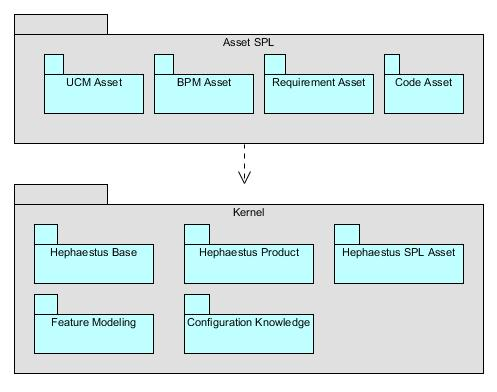
\includegraphics[width=.9\textwidth]{imagens/architecture-hpl-vf.jpg}
\end{center}
\caption{\hpl's architecture}
\label{fig:hpl-architecture}
\end{figure*}

%%%%%%%%%%%%%%%%%%%%%%%%%%%%%%%%%%%%%%%%%%%%%%%%%%

\subsection{\hpl's Architecture} 
\label{sec:hpl-architecture}

\hpl's architecture is depicted in Figure~\ref{fig:hpl-architecture}. Overall, \hpl{} is componentized in a way that most parts are separately compilable and unaffected by configuration or extension.

\emph{Kernel} represents the basic abstractions necessary for the generation of \hpl{} instances including the generation of \hpl{} itself in a bootstrapping process. Within the kernel, component \hpbase{} represents the commonality among all \hpl{} instances (as identified in Section~\ref{sec:commonality}); it serves as a base for deriving all \hpl{} instances. To this end, \hpbase{} has variability points (as identified in Section~\ref{sec:variability}) which are to be resolved by transformations defined in component \hpsplasset{} in a derivation process driven by component \hpproduct. These components of the kernel had to be specifically designed and implemented for \hpl. The kernel also hosts \emph{Feature Modeling} and \emph{Configuration Knowledge}: these components provide
basic abstractions for the representation of feature models, feature configurations, configuration knowledge as well as associated support functionality, e.g., for verifying validity of feature configurations relative to a given feature model. These components of the kernel could be reused from \hp{} and all \hpl{} instances share them, as is.

\textit{SPL Assets} represents the assets of \hpl. Each such \emph{meta-level} asset essentially corresponds to a type of artifact that can be targeted with an \hpl{} instance including the corresponding (non-meta-level) asset base for the type and designated support for variability management and product derivation in the domain of the asset. Each meta-level asset is essentially packaged in a component that exposes abstractions corresponding to the variation points of Section~\ref{sec:variability}: datatypes for the representation of assets and their transformation, functions for the interpretation of transformations, and other functionality related to \hpl's feature model, notably export functions.

%%%%%%%%%%%%%%%%%%%%%%%%%%%%%%%%%%%%%%%%%%%%%%%%%%

\subsection{\hpl's Transformational Approach} 
\label{sec:hpl-transformation}

We adopt a transformational approach~\cite{deltaSchaefer} to variability management. That is, the derivation of an \hpl{} instance involves source-code transformation. The approach provides transformations to address the heterogeneity of the variability patterns observed in Section~\ref{sec:hp-evolution} without compromising modularity and comprehensibility of \hpl, and thus configurability and extensibility, which may be issues for annotative approaches~\cite{kastner:2008}. The approach is also designed for uniformity. That is, the \hp{} approach to feature modeling, feature configuration, declaration and interpretation of configuration knowledge is adopted also at the meta-level. \hp{} often delegates some part of variability management to external tool support (e.g., for pre-processsing or aspect weaving), in which case, the transformation in the configuration knowledge essentially trigger those external transformations. In contrast, \hpl{} fully implements the meta-level transformations as metaprograms in Haskell on top of object programs in Haskell.

%%%%%%%%%%%%%%%%%%%%%%%%%%%%%%%%%%%%%%%%%%%%%%%%%%

\begin{figure}[t!]
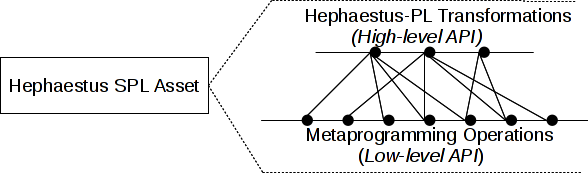
\includegraphics[scale=0.7]{imagens/apis-hpl-asset.png}
\caption{API levels for \hpsplasset}
\label{fig:hpl-apis}
\end{figure}

%%%%%%%%%%%%%%%%%%%%%%%%%%%%%%%%%%%%%%%%%%%%%%%%%%

Configuration of \hpl{} relies on transformations provided by a high-level API, which are implemented in terms of 
transformations of a low-level API, which, in turn, are implemented in terms of metaprogramming operations (with Haskell used both for object- and metaprograms).  The design of the high-level API captures the variability as identified during the domain analysis (Section~\ref{sec:variability}). The low-level API captures adaptation patterns as identified during the examination of the evolution scenario (Section~\ref{sec:hp-evolution}). Figure~\ref{fig:hpl-apis} illustrates the API layers, as they are part of \hpl's component \hpsplasset{} in the \emph{Kernel}. We refer to  Section~\ref{sec:metaprogrammingOperations} for the description of the actual implementation.

The transformations of the high-level API are of specific interest from the point of view of domain design, as these transformations are directly used in the configuration of \hpl. A description follows. (Some details specific to bootstrapping are deferred until Section~\ref{sec:hpl-bootstrapping}.)

\begin{description}

\item[SelectBase] selects \hpbase{}, which represents the commonality of all \hpl{} instances.
Typically, this is the first transformation to be executed in the process of deriving an instance. The implementation of \hpbase{} is given in Section~\ref{sec:hpbase}.

\item[BindProductName] sets the module name of the \hpl{} instance.

\item[SelectAsset] refines the product being derived with support for the selected asset, thereby enabling variability management for the associated type of artifacts. Technically, the transformation extends datatypes and functions for \assetr, \assetx, \asseti, \assetc, \emptyi, and \ckparser. To this end, existing extension points are connected with asset-specific abstractions and the underlying modules are added to the product.

\item[SelectExport] refines the product being derived with support for the selected couple of output format and asset. To this end, the transformation extends datatypes and functions for \asseto{} in a manner very similar to \emph{SelectAsset}. 

\end{description}

%%%%%%%%%%%%%%%%%%%%%%%%%%%%%%%%%%%%%%%%%%%%%%%%%%

\begin{table}[t!]
\begin{center}
\begin{tabular}{||l||l||}
  \hline
  \textbf{Feature Expressions} & \textbf{Transformations}   \\  \hline
  True & SelectBase \\  \hline
%  Hephaestus & BindProductName "Hephaestus" \\
%             &  SelectAsset "Hephaestus"   \\
%             &  RemoveProductMainFunction \\ \hline
%  NOT Hephaestus & SelectCKParser \\ \hline
  UseCase & SelectAsset "Use Case" \\ \hline
  UseCase AND UcmToXML & SelectExport "UcmToXML"  \\ \hline
  UseCase AND UcmToLatex & SelectExport "UcmToLatex" \\ \hline
  BusinessProcess & SelectAsset "Business Process" \\ \hline
  BusinessProcess AND BpmToXML & SelectExport "BpmToXML" \\ \hline
  Requirement & SelectAsset "Requirement" \\ \hline
  Requirement AND ReqToLatex & SelectExport "ReqToLatex" \\ \hline
  Code & SelectAsset "Code" \\ \hline
  Code AND BuildFile & SelectExport "BuildFile" \\ \hline
\end{tabular}
\caption{\hpl's configuration knowledge}
\label{tab:hpl-ck}
\end{center}
\end{table}

%%%%%%%%%%%%%%%%%%%%%%%%%%%%%%%%%%%%%%%%%%%%%%%%%%

\subsection{\hpl's Configuration Knowledge} 
\label{sec:hpl-ck}

Table~\ref{tab:hpl-ck} shows \hpl's configuration knowledge, without some details related to bootstrapping, which are deferred to Section~\ref{sec:hpl-bootstrapping}.

%%%%%%%%%%%%%%%%%%%%%%%%%%%%%%%%%%%%%%%%%%%%%%%%%%

\subsection{\hpl's Derivation Process} 
\label{sec:hpl-derivation}

%%%%%%%%%%%%%%%%%%%%%%%%%%%%%%%%%%%%%%%%%%%%%%%%%%

The derivation process evaluates the condition for each line of CK for the given feature configuration. 
In this manner, transformations with true conditions are collected; they are applied consecutively in the order, as they appear in the table, with the \emptyi{} serving as input for the first transformation and the final product corresponding to the output of the last transformation. 

%%%%%%%%%%%%%%%%%%%%%%%%%%%%%%%%%%%%%%%%%%%%%%%%%%

\begin{figure*}[t!]
\begin{center}
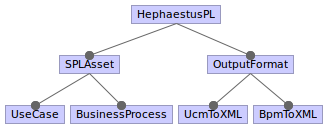
\includegraphics[scale=0.8]{imagens/fc-ucm-bpm.png}
\end{center}
\caption{An illustrative \hpl's feature configuration}
\label{fig:fc-ucm-bpm}
\end{figure*}

%%%%%%%%%%%%%%%%%%%%%%%%%%%%%%%%%%%%%%%%%%%%%%%%%%

Figure~\ref{fig:fc-ucm-bpm} shows a feature configuration which we use for the illustration of the derivation process. The configuration selects four features: use case models (\emph{UseCase}), business process models (\emph{BusinessProcess}), and both kinds models in XML format (\emph{UcmToXML} and \emph{BpmToXML}).

%%%%%%%%%%%%%%%%%%%%%%%%%%%%%%%%%%%%%%%%%%%%%%%%%%

\begin{figure*}[t!]
\begin{center}
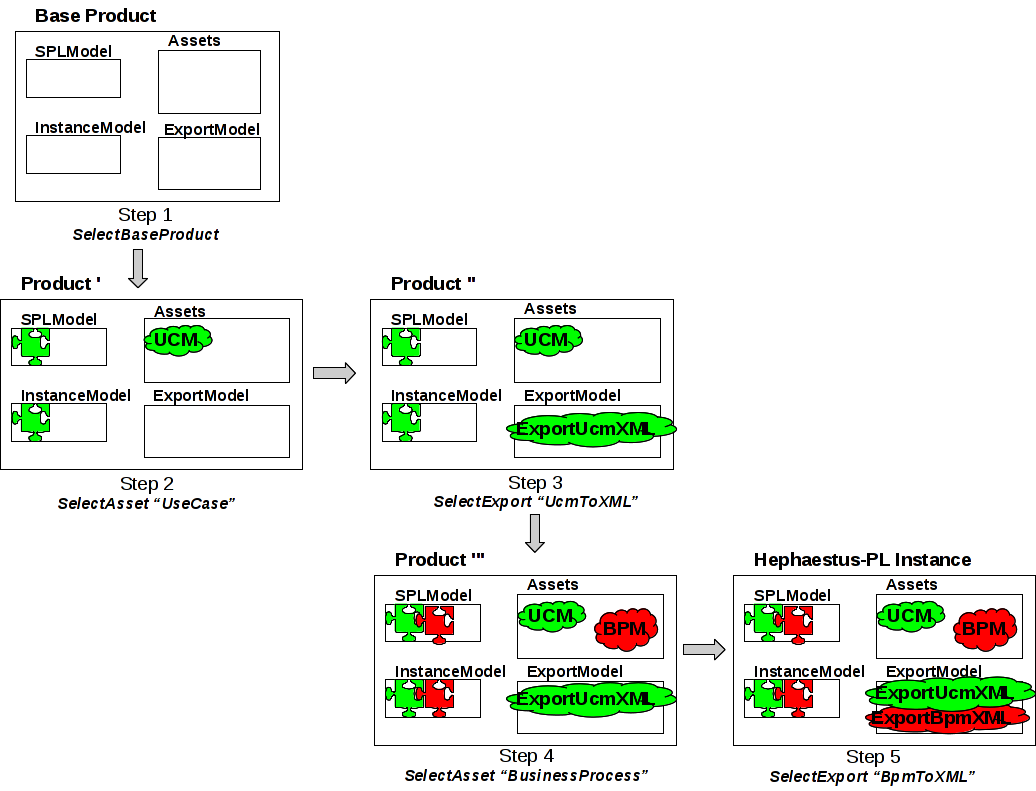
\includegraphics[width=\textwidth]{imagens/derivation.png}
\end{center}
\caption{Derivation of an \hpl{} instance supporting the UCM, BPM, UcmToXML and BpmToXML features}
\label{fig:hpl-derivation}
\end{figure*}

%%%%%%%%%%%%%%%%%%%%%%%%%%%%%%%%%%%%%%%%%%%%%%%%%%

Figure~\ref{fig:hpl-derivation} abstractly depicts the steps taken in \hpl's product derivation process 
for the feature configuration of Figure~\ref{fig:fc-ucm-bpm}. \hpl{}'s CK guides this transformational process in five steps towards the generation of a \hpl{} instance from the base product.

\hpl's product derivation process begins with the execution of the \texttt{SelectBase} transformation associated with the feature expression \texttt{True} in the first line of \hpl's CK (Table ~\ref{tab:ck-hpl}); see the first step in Figure~\ref{fig:hpl-derivation}. Next, the \emph{UseCase} feature expression in the second CK line evaluates to true for the feature configuration at hand and thus the \texttt{SelectAsset "Use Case"} transformation is executed; see the second step in Figure~\ref{fig:hpl-derivation}. In this manner, the \emph{UCM Asset} is incorporated into the product. 
Next, the \emph{UseCase AND UcmToXML} feature expression in the third CK line evaluates to true and thus the \texttt{SelectExport "UcmToXML"} transformation is executed; see the third step in Figure~\ref{fig:hpl-derivation}. In this manner, \asseto{} for the \emph{UCM Asset} is incorporated into the product. Another two steps handle the \emph{BPM Asset} very similar to the \emph{UCM Asset}.

%%%%%%%%%%%%%%%%%%%%%%%%%%%%%%%%%%%%%%%%%%%%%%%%%%

\subsection{Bootstrapping of \hpl} 
\label{sec:hpl-bootstrapping}

Consider again \hpl's architecture in Figure~\ref{fig:hpl-architecture}. \hpsplasset{} in the \emph{Kernel} provides datatypes and functions for representing and transforming \hpl{} products, i.e., tools for product derivation---in the same way as the components in the \emph{Asset SPL} provide datatypes and functions for regular assets. Thus, bootstrapping of \hpl, specifically derivation of \hpproduct, is relatively straightforward, as we discuss now.

%%%%%%%%%%%%%%%%%%%%%%%%%%%%%%%%%%%%%%%%%%%%%%%%%%

\begin{table}[t!]
\begin{center}
\begin{tabular}{||l||l||}
  \hline
  \textbf{Feature Expressions} & \textbf{Transformations}   \\  \hline
  Hephaestus & BindProductName "Hephaestus" \\
  Hephaestus & SelectAsset "Hephaestus"   \\
  Hephaestus & RemoveProductMainFunction \\ \hline
  NOT Hephaestus & SelectCKParser \\ \hline
\end{tabular}
\caption{Lines of \hpl's CK related to \hp{} feature}
\label{tab:hplck-2}
\end{center}
\end{table}

%%%%%%%%%%%%%%%%%%%%%%%%%%%%%%%%%%%%%%%%%%%%%%%%%%

\hpl's feature model contains a designated feature \hp, which is selected for bootstrapping. \hpl's configuration knowledge handles the feature in the manner shown in Table~\ref{tab:hplck-2}. The first two lines of CK directly model that bootstrapping builds \hpproduct{} from \hpsplasset.  That is, when the \hp{} feature is selected, the product name is set to be ``\hp'' and the ``\hp'' asset (i.e., \hpsplasset{} in the architecture) is selected. 

The last two lines are somewhat more idiosyncratic. The third lines models that \hpproduct{} uses a different (in fact, a much simpler) \texttt{main} function than other products. To this end, an extra transformation \emph{RemoveProductMainFunction} is invoked, with the simple intended semantics of removing the \texttt{main} for the product being derived. The fourth line models that \emph{CK parser} is only needed if features other than \hp{} are selected. To this end, an extra transformation \emph{SelectCKParser} is invoked, with the intended semantics of enhancing the product being derived such configuration knowledge is parsed, and passed as an argument to the \texttt{build} function. \hpproduct{} does not need \emph{CK Parser} because its configuration knowledge is defined as an abstraction as part of \hpsplasset; thus, parsing is not needed.

%%%%%%%%%%%%%%%%%%%%%%%%%%%%%%%%%%%%%%%%%%%%%%%%%%
